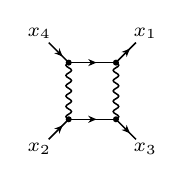
\begin{tikzpicture}[x=0.600cm, y=0.600cm, line width=0.550pt, baseline={([yshift=-0.6ex]0,0)}]
  \draw (-0.500,0.600) -- (0.500,0.600);
  \fill (0.089,0.600) -- (-0.089,0.676) -- (-0.031,0.600) -- (-0.089,0.524) -- cycle;
  \draw (-0.500,-0.600) -- (0.500,-0.600);
  \fill (0.089,-0.600) -- (-0.089,-0.524) -- (-0.031,-0.600) -- (-0.089,-0.676) -- cycle;
  \draw plot[smooth, tension=0.7] coordinates {(0.500,0.600) (0.542,0.573) (0.559,0.545) (0.542,0.518) (0.500,0.491) (0.458,0.464) (0.441,0.436) (0.458,0.409) (0.500,0.382) (0.542,0.355) (0.559,0.327) (0.542,0.300) (0.500,0.273) (0.458,0.245) (0.441,0.218) (0.458,0.191) (0.500,0.164) (0.542,0.136) (0.559,0.109) (0.542,0.082) (0.500,0.055) (0.458,0.027) (0.441,0.000) (0.458,-0.027) (0.500,-0.055) (0.542,-0.082) (0.559,-0.109) (0.542,-0.136) (0.500,-0.164) (0.458,-0.191) (0.441,-0.218) (0.458,-0.245) (0.500,-0.273) (0.542,-0.300) (0.559,-0.327) (0.542,-0.355) (0.500,-0.382) (0.458,-0.409) (0.441,-0.436) (0.458,-0.464) (0.500,-0.491) (0.542,-0.518) (0.559,-0.545) (0.542,-0.573) (0.500,-0.600)};
  \draw plot[smooth, tension=0.7] coordinates {(-0.500,-0.600) (-0.542,-0.573) (-0.559,-0.545) (-0.542,-0.518) (-0.500,-0.491) (-0.458,-0.464) (-0.441,-0.436) (-0.458,-0.409) (-0.500,-0.382) (-0.542,-0.355) (-0.559,-0.327) (-0.542,-0.300) (-0.500,-0.273) (-0.458,-0.245) (-0.441,-0.218) (-0.458,-0.191) (-0.500,-0.164) (-0.542,-0.136) (-0.559,-0.109) (-0.542,-0.082) (-0.500,-0.055) (-0.458,-0.027) (-0.441,0.000) (-0.458,0.027) (-0.500,0.055) (-0.542,0.082) (-0.559,0.109) (-0.542,0.136) (-0.500,0.164) (-0.458,0.191) (-0.441,0.218) (-0.458,0.245) (-0.500,0.273) (-0.542,0.300) (-0.559,0.327) (-0.542,0.355) (-0.500,0.382) (-0.458,0.409) (-0.441,0.436) (-0.458,0.464) (-0.500,0.491) (-0.542,0.518) (-0.559,0.545) (-0.542,0.573) (-0.500,0.600)};
  \draw (0.500,0.600) -- (0.924,1.024);
  \fill (0.796,0.896) -- (0.617,0.824) -- (0.711,0.811) -- (0.724,0.717) -- cycle;
  \draw (-0.500,-0.600) -- (-0.924,-1.024);
  \fill (-0.628,-0.728) -- (-0.807,-0.800) -- (-0.713,-0.813) -- (-0.700,-0.907) -- cycle;
  \draw (0.500,-0.600) -- (0.924,-1.024);
  \fill (0.796,-0.896) -- (0.724,-0.717) -- (0.711,-0.811) -- (0.617,-0.824) -- cycle;
  \draw (-0.500,0.600) -- (-0.924,1.024);
  \fill (-0.628,0.728) -- (-0.700,0.907) -- (-0.713,0.813) -- (-0.807,0.800) -- cycle;
  \fill (0.500,0.600) circle (0.064);
  \fill (-0.500,-0.600) circle (0.064);
  \fill (0.500,-0.600) circle (0.064);
  \fill (-0.500,0.600) circle (0.064);
  \node[font=\scriptsize, inner sep=0pt, anchor=225] at (0.988,1.088) {$x_{1}$};
  \node[font=\scriptsize, inner sep=0pt, anchor=45] at (-0.988,-1.088) {$x_{2}$};
  \node[font=\scriptsize, inner sep=0pt, anchor=135] at (0.988,-1.088) {$x_{3}$};
  \node[font=\scriptsize, inner sep=0pt, anchor=315] at (-0.988,1.088) {$x_{4}$};
\end{tikzpicture}
\allowbreak\;{-}\; 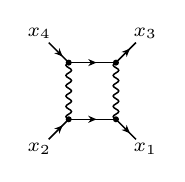
\begin{tikzpicture}[x=0.600cm, y=0.600cm, line width=0.550pt, baseline={([yshift=-0.6ex]0,0)}]
  \draw (-0.500,-0.600) -- (0.500,-0.600);
  \fill (0.089,-0.600) -- (-0.089,-0.524) -- (-0.031,-0.600) -- (-0.089,-0.676) -- cycle;
  \draw (-0.500,0.600) -- (0.500,0.600);
  \fill (0.089,0.600) -- (-0.089,0.676) -- (-0.031,0.600) -- (-0.089,0.524) -- cycle;
  \draw plot[smooth, tension=0.7] coordinates {(0.500,-0.600) (0.458,-0.573) (0.441,-0.545) (0.458,-0.518) (0.500,-0.491) (0.542,-0.464) (0.559,-0.436) (0.542,-0.409) (0.500,-0.382) (0.458,-0.355) (0.441,-0.327) (0.458,-0.300) (0.500,-0.273) (0.542,-0.245) (0.559,-0.218) (0.542,-0.191) (0.500,-0.164) (0.458,-0.136) (0.441,-0.109) (0.458,-0.082) (0.500,-0.055) (0.542,-0.027) (0.559,0.000) (0.542,0.027) (0.500,0.055) (0.458,0.082) (0.441,0.109) (0.458,0.136) (0.500,0.164) (0.542,0.191) (0.559,0.218) (0.542,0.245) (0.500,0.273) (0.458,0.300) (0.441,0.327) (0.458,0.355) (0.500,0.382) (0.542,0.409) (0.559,0.436) (0.542,0.464) (0.500,0.491) (0.458,0.518) (0.441,0.545) (0.458,0.573) (0.500,0.600)};
  \draw plot[smooth, tension=0.7] coordinates {(-0.500,-0.600) (-0.542,-0.573) (-0.559,-0.545) (-0.542,-0.518) (-0.500,-0.491) (-0.458,-0.464) (-0.441,-0.436) (-0.458,-0.409) (-0.500,-0.382) (-0.542,-0.355) (-0.559,-0.327) (-0.542,-0.300) (-0.500,-0.273) (-0.458,-0.245) (-0.441,-0.218) (-0.458,-0.191) (-0.500,-0.164) (-0.542,-0.136) (-0.559,-0.109) (-0.542,-0.082) (-0.500,-0.055) (-0.458,-0.027) (-0.441,0.000) (-0.458,0.027) (-0.500,0.055) (-0.542,0.082) (-0.559,0.109) (-0.542,0.136) (-0.500,0.164) (-0.458,0.191) (-0.441,0.218) (-0.458,0.245) (-0.500,0.273) (-0.542,0.300) (-0.559,0.327) (-0.542,0.355) (-0.500,0.382) (-0.458,0.409) (-0.441,0.436) (-0.458,0.464) (-0.500,0.491) (-0.542,0.518) (-0.559,0.545) (-0.542,0.573) (-0.500,0.600)};
  \draw (0.500,-0.600) -- (0.924,-1.024);
  \fill (0.796,-0.896) -- (0.724,-0.717) -- (0.711,-0.811) -- (0.617,-0.824) -- cycle;
  \draw (-0.500,-0.600) -- (-0.924,-1.024);
  \fill (-0.628,-0.728) -- (-0.807,-0.800) -- (-0.713,-0.813) -- (-0.700,-0.907) -- cycle;
  \draw (0.500,0.600) -- (0.924,1.024);
  \fill (0.796,0.896) -- (0.617,0.824) -- (0.711,0.811) -- (0.724,0.717) -- cycle;
  \draw (-0.500,0.600) -- (-0.924,1.024);
  \fill (-0.628,0.728) -- (-0.700,0.907) -- (-0.713,0.813) -- (-0.807,0.800) -- cycle;
  \fill (0.500,-0.600) circle (0.064);
  \fill (-0.500,-0.600) circle (0.064);
  \fill (0.500,0.600) circle (0.064);
  \fill (-0.500,0.600) circle (0.064);
  \node[font=\scriptsize, inner sep=0pt, anchor=135] at (0.988,-1.088) {$x_{1}$};
  \node[font=\scriptsize, inner sep=0pt, anchor=45] at (-0.988,-1.088) {$x_{2}$};
  \node[font=\scriptsize, inner sep=0pt, anchor=225] at (0.988,1.088) {$x_{3}$};
  \node[font=\scriptsize, inner sep=0pt, anchor=315] at (-0.988,1.088) {$x_{4}$};
\end{tikzpicture}